\documentclass{article}

% optional packages
\usepackage[utf8]{inputenc}
\usepackage{hyperref}
\usepackage{url}
\usepackage{booktabs}
\usepackage{amsfonts}
\usepackage{microtype}
\usepackage{graphicx}
\usepackage{subfig}
\usepackage{algorithm, algorithmic}

% pass options to natbib (if needed) before loading dai_2019
% \PassOptionsToPackage{authoryear,sort&compress}{natbib}

% for camera-ready version:
\usepackage[final]{dai_2019} 
% for submission:
% \usepackage{dai_2019}

% your custom packages, macros, etc.

\title{Compressed Suffix Memory Algorithm for Reinforcement Learning%\thanks{Title notes.}
}

% Please use \And between authors, or use \AND to force line breaking.

\author{%
  Feng Liu\\ 
  Nanjing University\\ 
  Nanjing, China \\
  \texttt{fengliu@nju.edu.cn} \\
  % more authors
  \And
  Haomin Qiu \\
  Nanjing University\\ 
  Nanjing, China \\
  \texttt{aquafits@outlook.com} \\
  \And
  Peng Huang \\
  Nanjing University\\ 
  Nanjing, China \\
  \texttt{paulwongpang@foxmail.com} \\
  \And
  Chongjun Wang \\
  Nanjing University\\ 
  Nanjing, China \\
  \texttt{chjwang@nju.edu.cn} \\
  % \And
  % Coauthor \\
  % Affiliation \\
  % Address \\
  % \texttt{email} \\
}

\begin{document}

\maketitle 

\begin{abstract}
  Instance-based approaches are effective ways to solve reinforcement learning problems.
  Utile Suffix Memory (USM) algorithm has shown decent results for distinguishing different
  states from instance chains and generating Q-value of actions of each state, but involving
  exponentially expanded state space and a number of redundant states. In this paper we
  propose a new state space compressed algorithm, called Compressed Suffix Memory (CSM)
  algorithm. CSM algorithm obtains heuristic information of the environment by a blind
  exploration, for example, the maximum L1 distance between instances in instance chains
  and goal frequencies, to improve efficiency and resist overfitting. Boltzmann sampling
  is adopted to balance between exploration and exploitation. Experiments show that both
  the efficiency and the effect have been improved a lot by CSM algorithm compared with
  USM algorithm.
\end{abstract}

\section{Introduction}

Reinforcement learning is learning what to do—how to map situations to actions—so
as to maximize a numerical reward signal in a provided environment
\cite{sutton2018reinforcement}. In many reinforcement learning scenarios such as
robotic exploration \cite{smith2007probabilistic} and autonomous driving
\cite{bai2015intention}, the agent is only able to gain partial and noisy
observations form environment, so POMDP (partially observable Markov decision
process) model is wildly adopted. According to the observations, reward and the
historical information, POMDPs provide a rich mathematical approach to solving
sequential problems by calculating the Q-value of actions.

As the agent does not directly observe the underlying state, the generation of
the state space is the key to reinforcement learning algorithms.
Many instance-based methods have been put forward, including Nearest Sequence
Memory (NSM) algorithm \cite{mccallum1997reinforcement} and Utile Suffix Memory
(USM) algorithm \cite{mccallum1995instance}. USM algorithm presents the state space by
tree-nodes in a suffix tree building from the instance chains, and is proved
effective maximizing the Q-value of actions. However, the state space of USM
algorithm exponentially expands during iteration and comprises many redundant
states, which reduces the efficiency. Furthermore, because the $\epsilon$-greedy
policy of USM lacks of the exploitation of overall information, it may lead to
overfitting.

In this paper, we propose a new algorithm, called Compressed Suffix Memory (CSM)
algorithm, which optimizes the generation of a utile tree and decision process.
First, the heuristic information is obtained by the blind exploration
of the environment, e.g., $l$ as the effective path length from start to goal
and $p$ as the probability of goal during the exploration. Second, the maximum
depth of the suffix tree is limited to $2l$ and the minimum instances required
to trigger state splitting, the threshold $b$, is deduced from $p$. Finally, after initializing the agent
with a random policy, Boltzmann sampling approach will be applied. Experiment has shown
that both the efficiency and the effect have been greatly improved by CSM algorithm compared
with USM algorithm.

The paper outline follows. We will briefly review reinforcement in partially observable
environment and Utile Suffix Memory (USM) algorithm, in Section 2.
Next, we propose Compressed Suffix Memory (CSM) algorithm, which takes advantage of
heuristic information and optimizes the generation of the suffix tree, in Section 3.
We measure the performance of CSM algorithm and see improvements comparing with USM algorithm, in Section 4.
We close in Section 5, with a brief summary and possible means of improvement of CSM algorithm.

\section{Background}

\subsection{Reinforcement Learning in Partially Observable Environment}

Reinforcement learning is about how an agent learning to map states to actions
and produce a maximized reward in a provided environment. In general, a
reinforcement learning agent interacts with the environment over time.
At each time step $t$, it determines its state $s_t$ from a state space $S$,
and chooses a best action $a_t$ from an action space $A$ according to the policy
$\pi$. The agent gets an instant reward $r_t$ according to the reward function
$R(s_t, a_t)$ and transfer to the next state $s_{t+1}$ according to the transition
probability $T(s_{t+1}|s_t, a_t)$. The reward is normally discounted with factor
$\gamma\in(0,1]$, and the   accumulated reward at $t_n$ is defined as
$R_{t_n}=\sum_{t=0}^{t_n} \gamma^t r_t$. When a problem satisfies the Markov
property, the problem can be formulated as a Markov decision process (MDP), which
is defined by the 5-tuple ($S, A, T, R, \gamma$).

However, in most cases, an agent cannot directly observe the states of the
underlying MDP model in the provided environment, but can only deduce a state by an
observation. It is necessary to bring in partially observable Markov decision
process (POMDP). It defines $\Omega$ as a set of observations and $O$ as a set of
conditional observation probabilities-mapping current state $s_t$ and
previous action $a_{t-1}$ to the probability of current observation $o_t$. 
In that way, a POMDP can be defined by the 7-tuple ($S, A, T, R, \Omega, O, \gamma$).

When the model is successfully learned, i.e., all elements of the 7-tuple are
generated to fit the problem, there are plenty of algorithms to calculate a best
policy \cite{shani2013survey}. However, in model-free methods, an agent can learn
with trail-and-error from experience directly and a policy can generated before
grasping all information of a model \cite{li2017deep}, which is normally faster
and more suitable real time problem.  An important way to implement model-free
methods is to make an agent comprise some sort of internal memory \cite{aberdeen2003policy,
meuleau1999learning, mccallum1995instance} (see Figure~\ref{fig:agent memory}).
For example, the states of a model can be expressed by some nearest observations
and internal states of an agent. After learning the state space, the agent can make
decisions using model-free methods, such as HQ-learning \cite{wiering1997hq}.

\begin{figure}[h]
  \centering
    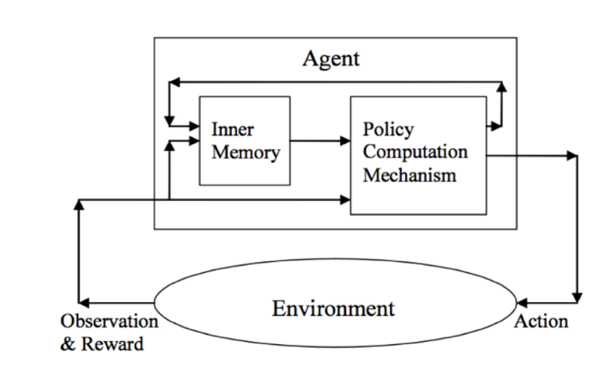
\includegraphics[width=0.45\textwidth]{agent_with_memory.png}
  \caption{The agent model that has internal memory}
  \label{fig:agent memory}
\end{figure}

The internal memory of an agent can comprise instances that record what it has
encountered at each time step. Nearest Sequence Memory (NSM) and Utile
Suffix Memory (USM) algorithms are based on the instances.


\subsection{Utile Suffix Memory Algorithm}

The interaction between the agent implementing USM algorithm and the environment is described by
$A, O, R$, which are finite set of actions, finite set of observations and a reward function.
Like other instance-based algorithms, USM algorithm records each of its raw instances
\cite{mccallum1995instance}. At each time step $t$, the agent executes action
$a_t \in A$ to get a new instance, gets observation $o_{t+1} \in O$, and get a
instant reward $r_{t+1}$ according to $R$, which is determined by the environment.
A new instance is formulated as
\begin{equation}
  T_{t+1}= (T_t, a_t, o_{t+1}, r_{t+1}). \label{equ:instance}
\end{equation}
$T_{t+1}$ is $T_t$'s successor. It is obvious that instance chains are built
from during learning process.

In order to deduce state space from those instance chains, USM algorithm creates a suffix tree,
whose leaves present the state space and store clustered instances. Each node of the tree
can thus be uniquely identified by the string of labels on the path from node to the root,
and the string is called the node’s suffix. An instance is always deposited into the
nodes whose suffix matches its observation and action context, or suffix. That is,
for an instance $T_i$, if its suffix $[..., o_{t-3}, a_{t-3}, o_{t-2}, a_{t-2}, o_{t-1}, a_{t-1}]$
matches the suffix of a certain node, it would be put into that node (see Figure~\ref{fig:suffix tree}).
The set of instances that a node contains is written as $I(s)$. The suffix tree leaf which
instance $T$ belongs to is written as $L(T)$. It is inevitable that the action layer and
the observation layer appears alternately when tree grows (see Figure~\ref{fig:suffix tree}).

\begin{figure}[h]
  \centering
    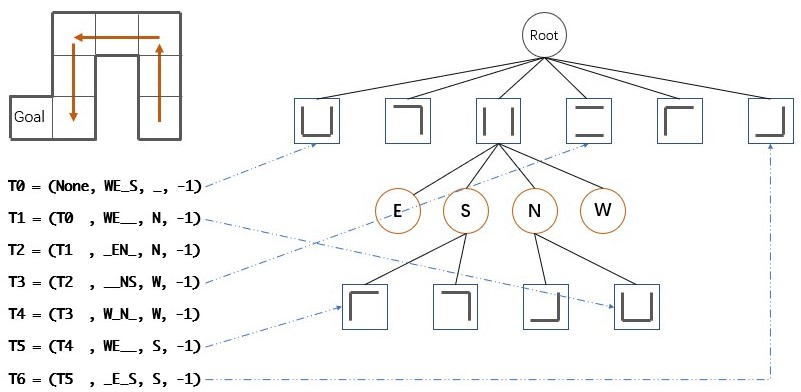
\includegraphics[width=0.45\textwidth]{usm_sample.jpg}
  \caption{The agent navigates itself in a maze (probably not the first time), generates
  a sequence of instances, and builds a suffix tree. The action layer and
  the observation layer appear alternately.}
  \label{fig:suffix tree}
\end{figure}

Besides the general nodes, there is another type of node called "fringe" node \cite{mccallum1995instance}.
The fringe nodes are actually the deepest layers of the suffix tree, however, we treated them
the inner instance buckets of the leaves previously mentioned. Fringe nodes also contain
instances according to the same suffix criterion used by non-fringe nodes. That is, 
if the suffix of a leaf is $[a_{t-2}, o_{t-1}, a_{t-1}]$, an 1-layer deeper fringe nodes of it
will stores the instance that matches suffix $[o_{t-2}, a_{t-2}, o_{t-1}, a_{t-1}]$. The agent decides
whether it should promote fringe nodes to leaves by Kolmogorov-Smirnov test, which determine the
instances in the fringes and that of their parent are drawn the same distribution.

The steps of USM algorithm is as below:

\begin{enumerate}
  \item The agent begins with a suffix tree that comprises a root node and a layer of
  observation nodes as leaves, i.e., the agent only acts according to its observation.

  \item The agent chooses an action according to $\epsilon$-greedy policy, executes it and
  generates an instance (see Equation ~\ref{equ:instance}).

  \item The agent inserts the instance into the suffix tree. The instance is classified to
  leaves and fringes with the same suffix with that instance. 

  \item The agent triggers K-S test every $n$ additions of instance. If the Q-value of fringes
  and their parent are from different distributions, the fringes will be promoted to leaves.
  The instance will always be added to fringes and leaves that have the same suffix with the instance.
  Q-value table will be updated after every addition of instance. Time step increases and algorithm
  jumps to step 2.
\end{enumerate}

There are two obvious deficiencies of USM algorithm. Firstly, in USM algorithm,
the number of states may exponentially increase as the number of steps grows, but many
states are redundant, which correspond to the same state in the real environment. Thus, it
will reduce the efficiency of the algorithm. Secondly, since the initial Q value of all leaves
is initialized with 0, the $\epsilon$-greedy policy may lead to overfitting. Because
the $\epsilon$-greedy policy of USM treats the second best and the worst the same, it drastically
decrease the probability to explore other actions which may get higher reward. For example,
we found that in the first few steps, the agent may get negative default return after
choosing actions at some states, which decreases the probability of exploring those actions
when at those states again.

\section{Compressed Suffix Memory Algorithm}

Exploration and exploitation is a key issue in reinforcement learning. Heuristic information
of environment can help agent understand state space better. Agent could first make a blind
policy exploration of the environment, obtaining some interaction experience, and apply
it to following reinforcement learning. The effective path length to goal and the frequency
of goals decently represents the scale of the environment and can be used to improve the algorithm.
In addition, more overall information should be considered.

\begin{enumerate}
  \item The depth of the suffix tree should be constrained. The $3^\textnormal{rd}$ Quartile of
  path lengths to goal and the maximum tree depth are denoted as $l_3$ and $d$. Leaves with suffix longer
  than $2l_3$ are considered redundant. However, the exploitation of immature policy can cause overfitting,
  which makes $d$ grows greater than $2l_3$. So, an alterable guardian depth $l$ is needed.
  On the one hand, $l$ starts with a relatively small value and will gradually get closer
  to $l_3$ through learning. On the other hand, $2l$ should always greater than $d$.
  The initial $l$ is set as:
  \begin{equation}
    l = \max{L_T}/2,
  \end{equation}
  and will be updated as:
  \begin{equation}
    l \leftarrow l + \alpha (l_3 - l)  \ s.t. \ l + \alpha (l_3 - l)> d/2. \label{equ:l3}
  \end{equation}
  $L_T$ is a set of L1 distances, which comprises the maximum L1 distance between each
  instance and the initial instance in each instance chain during the blind exploration;
  $\alpha$ is the learning rate.

  \item Instances in tree node should be denser. K-S test performs better with more statistical
  sample. Agent should only trigger K-S test when leaves and their fringe nodes are holding enough
  instances, namely, more than a threshold $b$. Because the ideal $b$ varies with environment itself.
  In practice, as the frequency of goal in blind exploration, $p$, well describes the problem scale,
  $b$ is strongly correlated with $p$. Agent is encouraged to match longer suffix when
  problem scale is bigger. Therefore, the smaller the $p$ is, the smaller the $b$ is set.

  \item More overall information should be taken into account. The main problem of
  $\epsilon$-greedy approach is that it lacks the exploitation of overall information,
  such as those Q-value which is not the maximum. We use Boltzmann sampling to balance between
  exploration and exploitation, which assigns actions with similar Q-value similar executing
  probabilities to encourage agent to exploit them all, rather than only the best.
  The probability to choose an action $a_i$ at leaf $s$ with temperature $t$ is
    \begin{equation}
      p(s, a_i) = e(s, a_i)/ \sum_a{e(s, a)} \label{equ:boltzmann},
    \end{equation}  
  which $e$ is
    \begin{equation}
      e(s, a) = \exp( (Q(s, a) - \max Q(s))/t )
    \end{equation}

\end{enumerate}

The details and the pseudo code (see Algorithm~\ref{alg:CSM}) form of CSM algorithm is as below.

\begin{enumerate}

  \item The agent begins with a suffix tree that comprises a root node and an layer of
  observation nodes as leaves, i.e., the agent only acts according to its observation.

  \item The agent is initialized with a randomly policy. The guardian length $l$ and
  minimum number of instances to do K-S test, $b$, are set during initialization. The
  maximum depth of the suffix tree is set to $2l$.

  \item The agent executes action and interacts with the environment at time step $t$.
  It records its learning history as an instance $T_t$ (see Equation~\ref{equ:instance}).
  For each treenode $s$, if its suffix matches the suffix of $T_t$. Its instance
  set are updated as:
    \begin{equation}
      I(s) \leftarrow I(s) \cup {T_t}.
    \end{equation}
  Let $L(T)$ be the leaf which instance $T$ belongs to. $L(T_t)$ is cached to agent memory.
  $l$ is updated (see Equation~\ref{equ:l3}). If the agent reaches the goal,
  it repositions itself randomly to one of the provided start positions, and updates
  the value of $l_3$.

  \item For each instance added, the agent does one Bellman iteration with the leaves of
  of the states:
    \begin{equation}
      Q(s,a) \leftarrow R(s,a)  + \gamma Pr(s'|s,a)U(s').
    \end{equation}
  Let $I(s,a)$ be the subset of $I(s)$ that contains all the instances that executed
  action $a$. $U(s')$ is the utility of the state $s'$, calculated as
  $U(s) = \max_{a \in A} Q(s,a)$. $R(s,a)$ and $Pr(s'|s,a)$ are the estimated immediate
  reward and the transition probability, respectively, that drawn from the instance chains:
    \begin{equation}
      R(s,a) = \frac{\sum_{T_i \in I(s,a)}r_i} {|I(s,a)|},
    \end{equation}

    \begin{equation}
      Pr(s'|s,a) = \frac{|\forall{T_i \in I(s,a) \ s.t. \ L(T_{i+1} = s')}|} {|I(s,a)|}.
    \end{equation}
  
  \item Kolmogorov-Smirnov is performed when $L(T_t)$ is not the same as $L(T_{t-1})$ and
  $L(T_t)$ holds enough instances (more than $b$). The expected discounted reward of instance
  $T_i$ is written as $H(T_i)$, and is defined as:
    \begin{equation}
      H(T_i) = r_i + \gamma U(L(T_{i+1}))
    \end{equation}
  Every $Q(T_i)$ of instances stored in leaf and those stored in immediate fringe nodes is
  calculated. Therefore, $|A|$ pairs of smaple are prepared for Kolmogorov-Smirnov test. If
  there existing a certain pair that is believed not from the same distribution, those
  fringe nodes would be promoted as leaves.

  \item Agent does Boltzmann sampling to choose the next action, i.e., with
  probability $p(s, a_i)$ the agent chooses $a_i$ as $a_{t+1}$ (see Equation~\ref{equ:boltzmann}).
  In practice, agent is encouraged to do random exploration for $n_r$ times, and then perform
  Boltzmann sampling method with descendant temperature.
  Time step increase to $t+1$ and algorithm jumps to step 3.
\end{enumerate}

\begin{algorithm}[h]
	\renewcommand{\algorithmicrequire}{\textbf{Input:}}
	\renewcommand{\algorithmicensure}{\textbf{Output:}}
	\caption{Compressed Suffix Algorithm}
	\label{alg:CSM}
	\begin{algorithmic}[1]
		\REQUIRE iteration steps $n$, radom steps in iteration $n_r$
		\ENSURE average discounted return $ADR$
    \STATE Initialize guardian length $l$, and minimum number $b$ of instance required to do K-S test
    by blind exploration
    \STATE Initialize temperature $t$ as positive infinity
    \STATE Initialize a suffix tree with depth limitation $2l$
    \STATE Initialize agent with random start position
		\FOR{$i=0$ to $n$}
		  \IF{$i>n_r$}
		    \STATE $t$ decreases from 0.5 to nearly 0 as $i$ increases
      \ENDIF

      \STATE Choose action $a$ by Boltzmann sampling and execute it (see Equation~\ref{equ:boltzmann})
      \WHILE{not moved after executed $a$}
        \STATE Choose action $a$ by Boltzmann sampling with higher $t$ and execute it
      \IF{the agent reaches goal}
		    \STATE Update $l_3$
      \ENDIF
      \ENDWHILE

      \STATE Generate instance $T$ according to the execution of $a$ just now
      \STATE Insert $T$ into the suffix tree, update $l$, and find the leaf node $s$ the instance belongs
      \STATE $I(s) = I(s) \cup {T_t}$
      \STATE $Q(s,a) = R(s,a) + \gamma Pr(s'|s,a)U(s')$
      \STATE $R(s,a) = {\sum_{T_i \in I(s,a)}r_i}/{|I(s,a)|}$
      \STATE $Pr(s'|s,a) = {|\forall{T_i \in I(s,a) \ s.t. \ L(T_{i+1} = s')}|} / {|I(s,a)|}$
      
      \IF {$|I(s)| > b$}
        \STATE do K-S test between $H(T)$s of $s$ and its fringe nodes, get p\_value $p$ 
        \IF {$p<0.1$}
          \STATE promote fringe nodes to leaves
        \ENDIF
      \ENDIF

      \IF {agent at goal}
        \STATE Initialize agent with random start position
      \ENDIF
    \ENDFOR
    \STATE Use Boltzmann sampling at low temperature on $Q(s, a)$ to produce average
    discounted reward $ADR$ (see Equation~\ref{equ:adr})
		\STATE \textbf{return} $ADR$
	\end{algorithmic}  
\end{algorithm}

\section{Experiment}

\subsection{Experiment Setup}

We run algorithms with three well-known benchmarks: Tiger-Grid, Hallway and McCallum 
as well as a large Prim Maze generated by Prim algorithm randomly
(see ~Figure \ref{fig:mazes}). The characteristics of benchmarks are described
below (see ~Table \ref{table:benchmarks}), where $|S|$, $|A|$, $|\Omega|$, $r_d$, $r_p$, $r_g$, 
denotes the number of states, the number of actions, the number of observations, default
reward, penalty and goal, respectively. The $|A|$ is 4 because the action of the agent
normally includes: moving south, west, east and north. However, problems differ in some
details.

\begin{figure}[h]
  \centering
    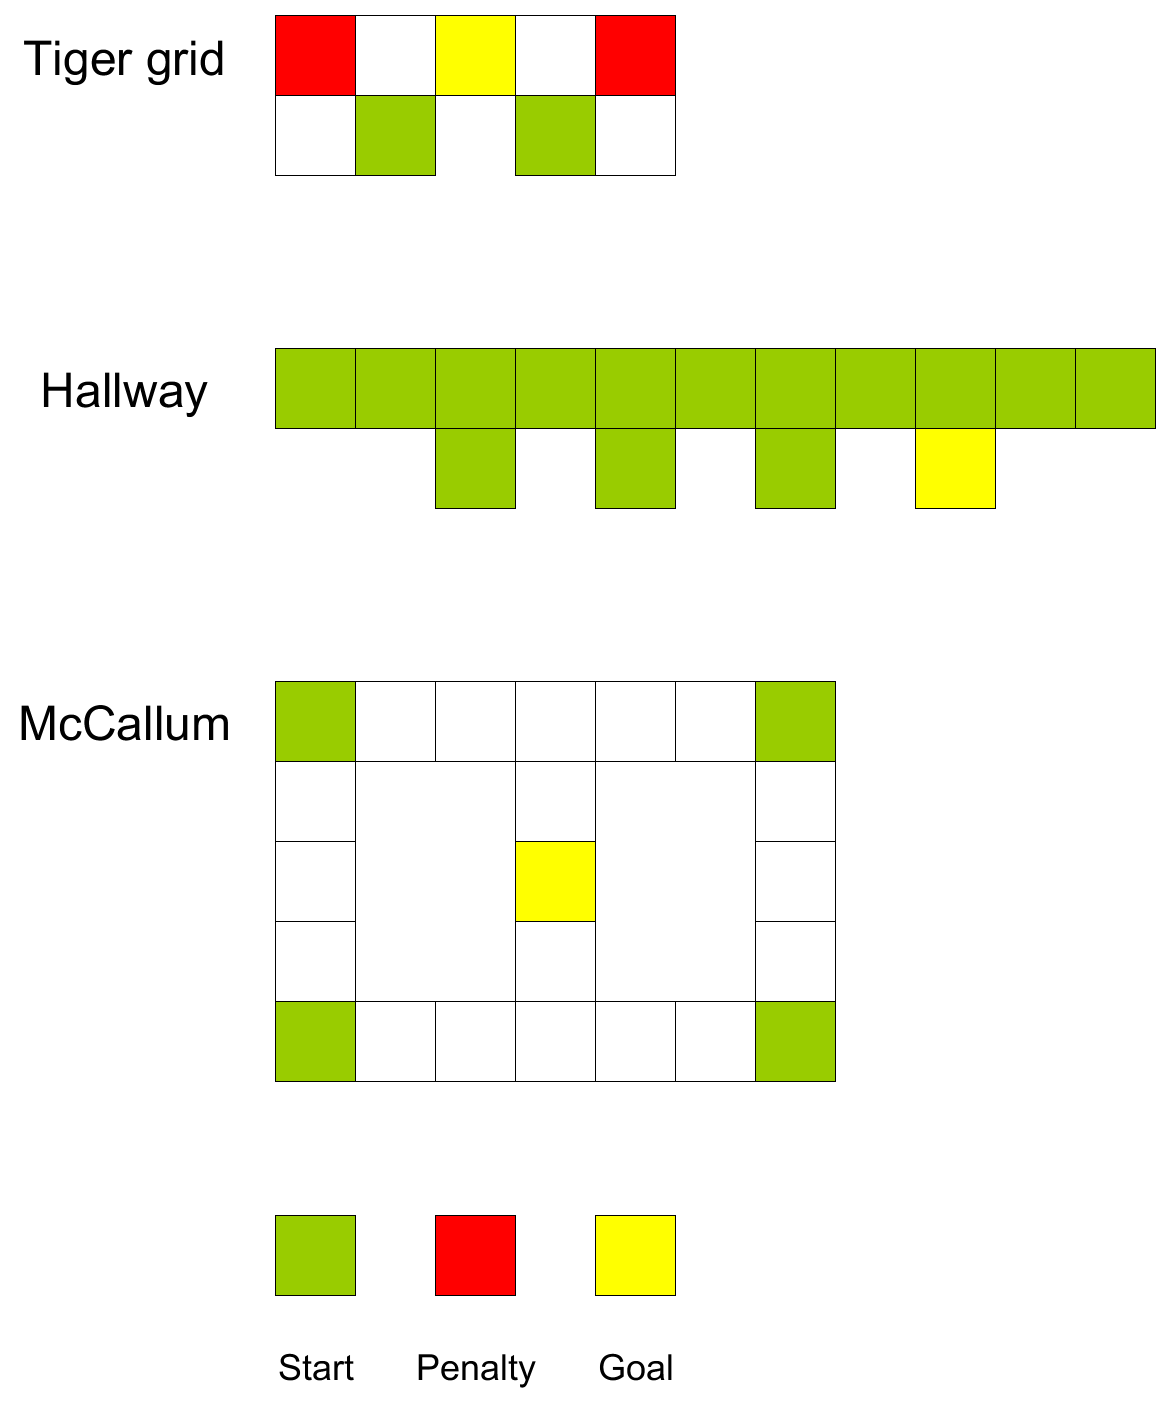
\includegraphics[width=0.45\textwidth]{mazes.png}
  \caption{Benchmark mazes}
  \label{fig:mazes}
\end{figure}

\begin{table}[h]
  \caption{Benchmarks}
  \label{table:benchmarks}
  \centering
  \begin{tabular}{lllllll}
    \toprule
    problem         & $|S|$          & $|A|$          & $|\Omega|$  &$r_d$  &$r_p$  &$r_g$\\
    \midrule
    Tiger-Grid      & 9              & 4              & 7           & -0.1  & -4    & 16  \\
    Hallway         & 15             & 4              & 4           & -0.1  &     & 32  \\
    McCallum        & 23             & 4              & 9           & -0.1  &     & 18  \\
    Prim Maze       & 154            & 4              & 16          & -0.1  &    & 96  \\
    \bottomrule
  \end{tabular}
\end{table}

In Tiger-Grid, the agents are initially assigned to one of two definite starting positions.
The probability of each starting position is 0.5. The goal of the model is to make the agent
reach the goal position as soon as possible. Once the agent reaches the goal position,
it will be reset to two starting positions. Tiger-Grid's maze comprises two penalty positions
where agent will receive a negative reward. 

In Hallway, similar to Tiger-Grid problem but still different, agent will be reset randomly
to a non-goal state. The Hallway does not include any penalty position. Furthermore, the hallway
adds 4 landmarks as hint for agent to discover hidden states.

In McCallum, after reached the goal, the agent will be randomly reset at one of the 4 corners.
There are 3 south-north hallways, which are deliberately designed for agent to distinguish, since
they are ambiguous. 

In Prim Maze, which is randomly generated by Prim algorithm and mean to be big. $|S|$ of Prim Maze
is several times the $S$ of others. When the agent arrives at the goal, Prim Maze will reset
the agent to a random state in the maze.

We evaluate average discounted reward, $ADR$, in the experiment:
\begin{equation}
  ADR = \frac{\sum_{i=0}^{n_{trails}} \sum_{j=0}^{n_{steps}} \gamma^j r^j}{n_{trails}}, \label{equ:adr}
\end{equation}
$n_{trails}$ is the number of trails we test our learning result; $n_{steps}$ is the maximum
steps to try to reach goal. $ADR$ is widely considered to be a good evaluation of the quality of
a value function. The higher the $ADR$ is, the more intelligent the agent is considered to be.
We track the changing of $ADR$ through time to determine whether CSM algorithm helps the agent to learn
faster and better.
  
Our experiment uses a discount factor $\gamma=0.9$, an exploration probability $\epsilon=0.1$ for USM algorithm.
The boundary value of the Kolmogorov-Smirnov test is $p=0.1$. We iterate the USM, CSM and random algorithm
2048 times, and set check points per 48 iteration. In each check point we test our model 256 times
within 96 steps, i.e., $n_{trial}$ is 256 (see Equation~\ref{equ:adr}) in $ADR$ calculation.

\subsection{Experiment Results}

The experiment results of CSM, USM and random algorithms are shown below (see Figure~\ref{fig:agent_adr_time}).
It should be noted that even if $n_trail$-set to 256-seems large enough, the results of $ADR$ may still fluctuate.
Therefore, we record ($ADR$, time) tuples in the table below (see Table \ref{table:results}), when $ADR$ starts
to become relatively stationary, rather than when $ADR$ gets maximum. 

\begin{figure}[!h]
	\centering
	\subfloat[Tiger Grid]{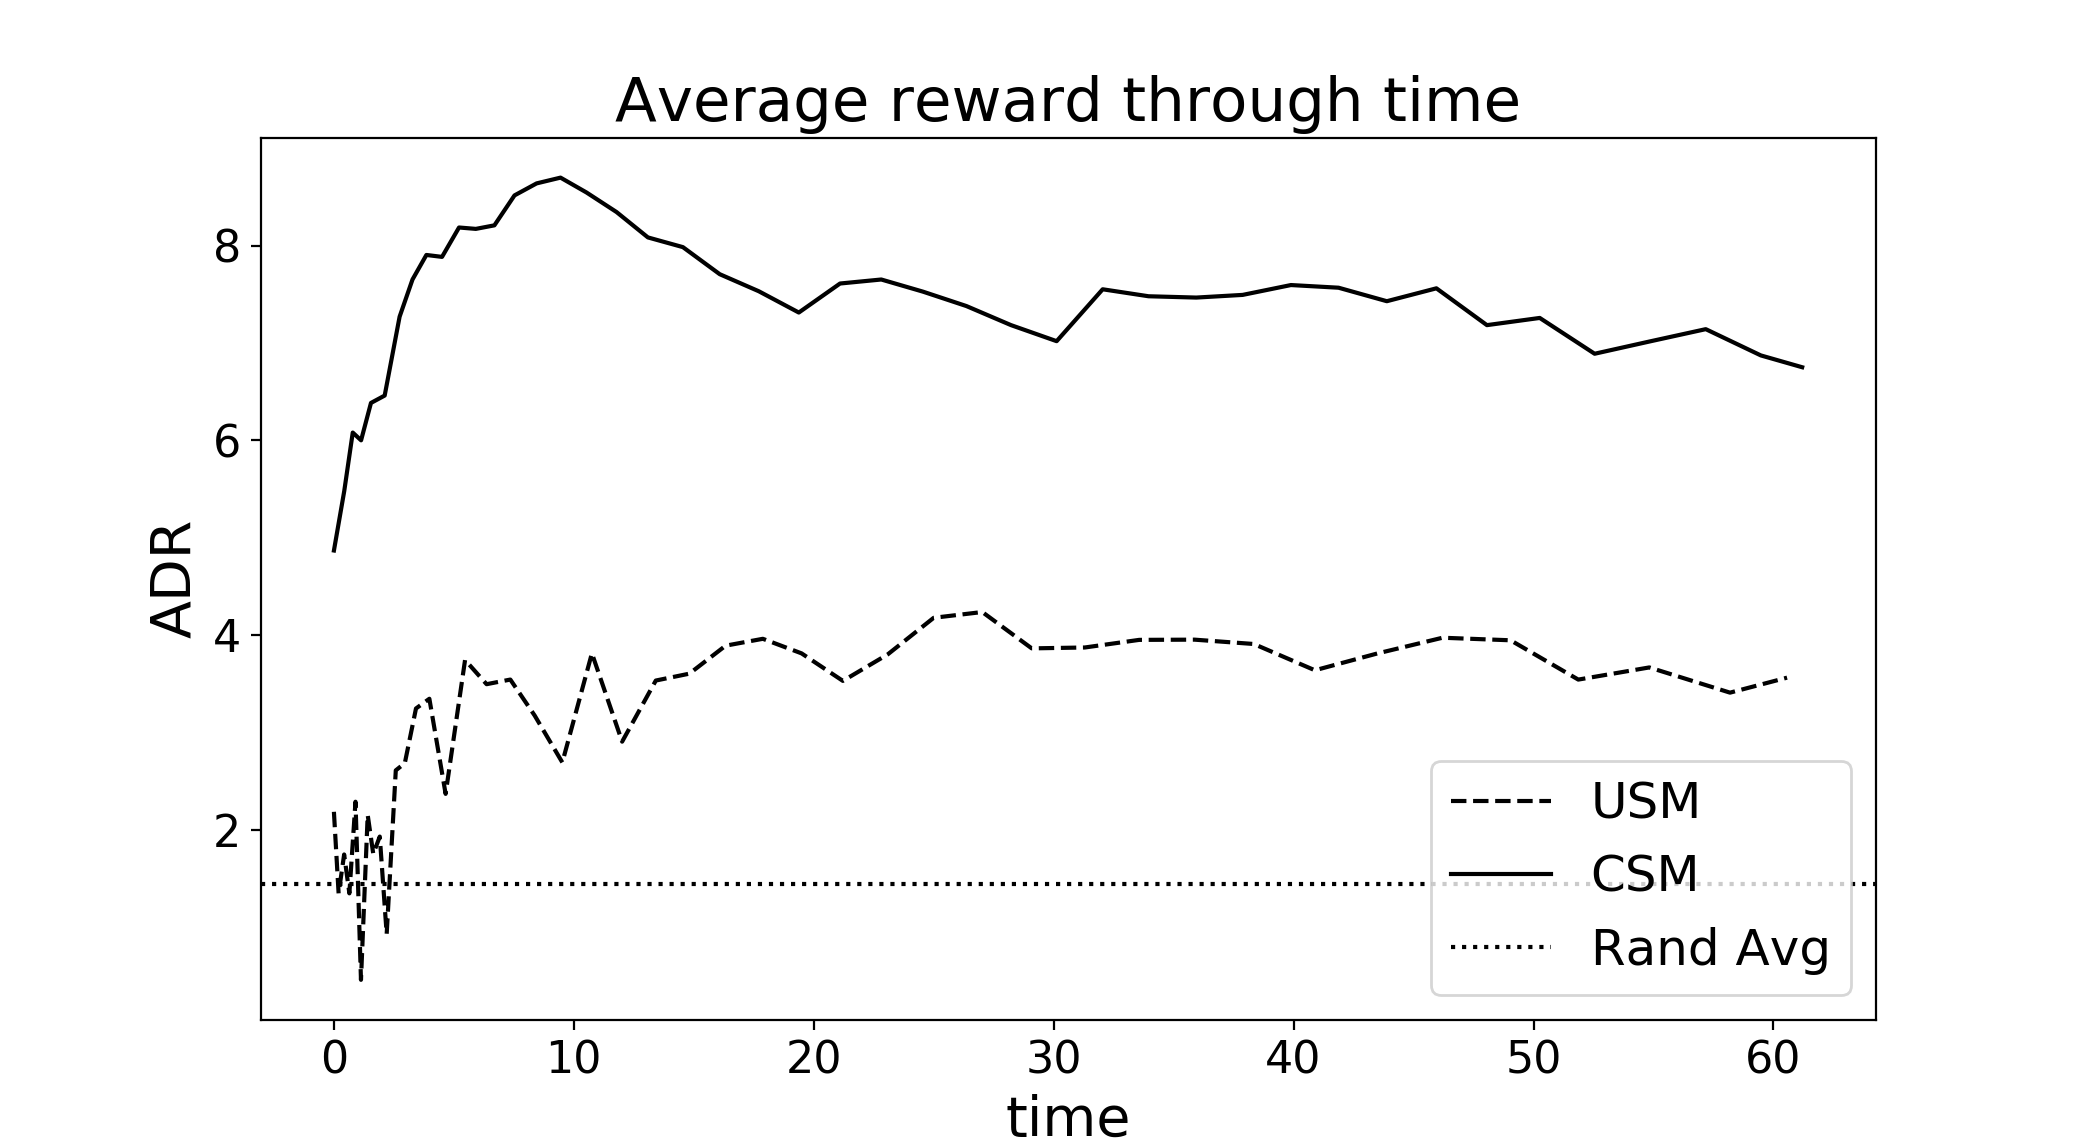
\includegraphics[width=2.8in]{06-13-21-48/tiger_grid_result.png}}\\
 \subfloat[Hallway]{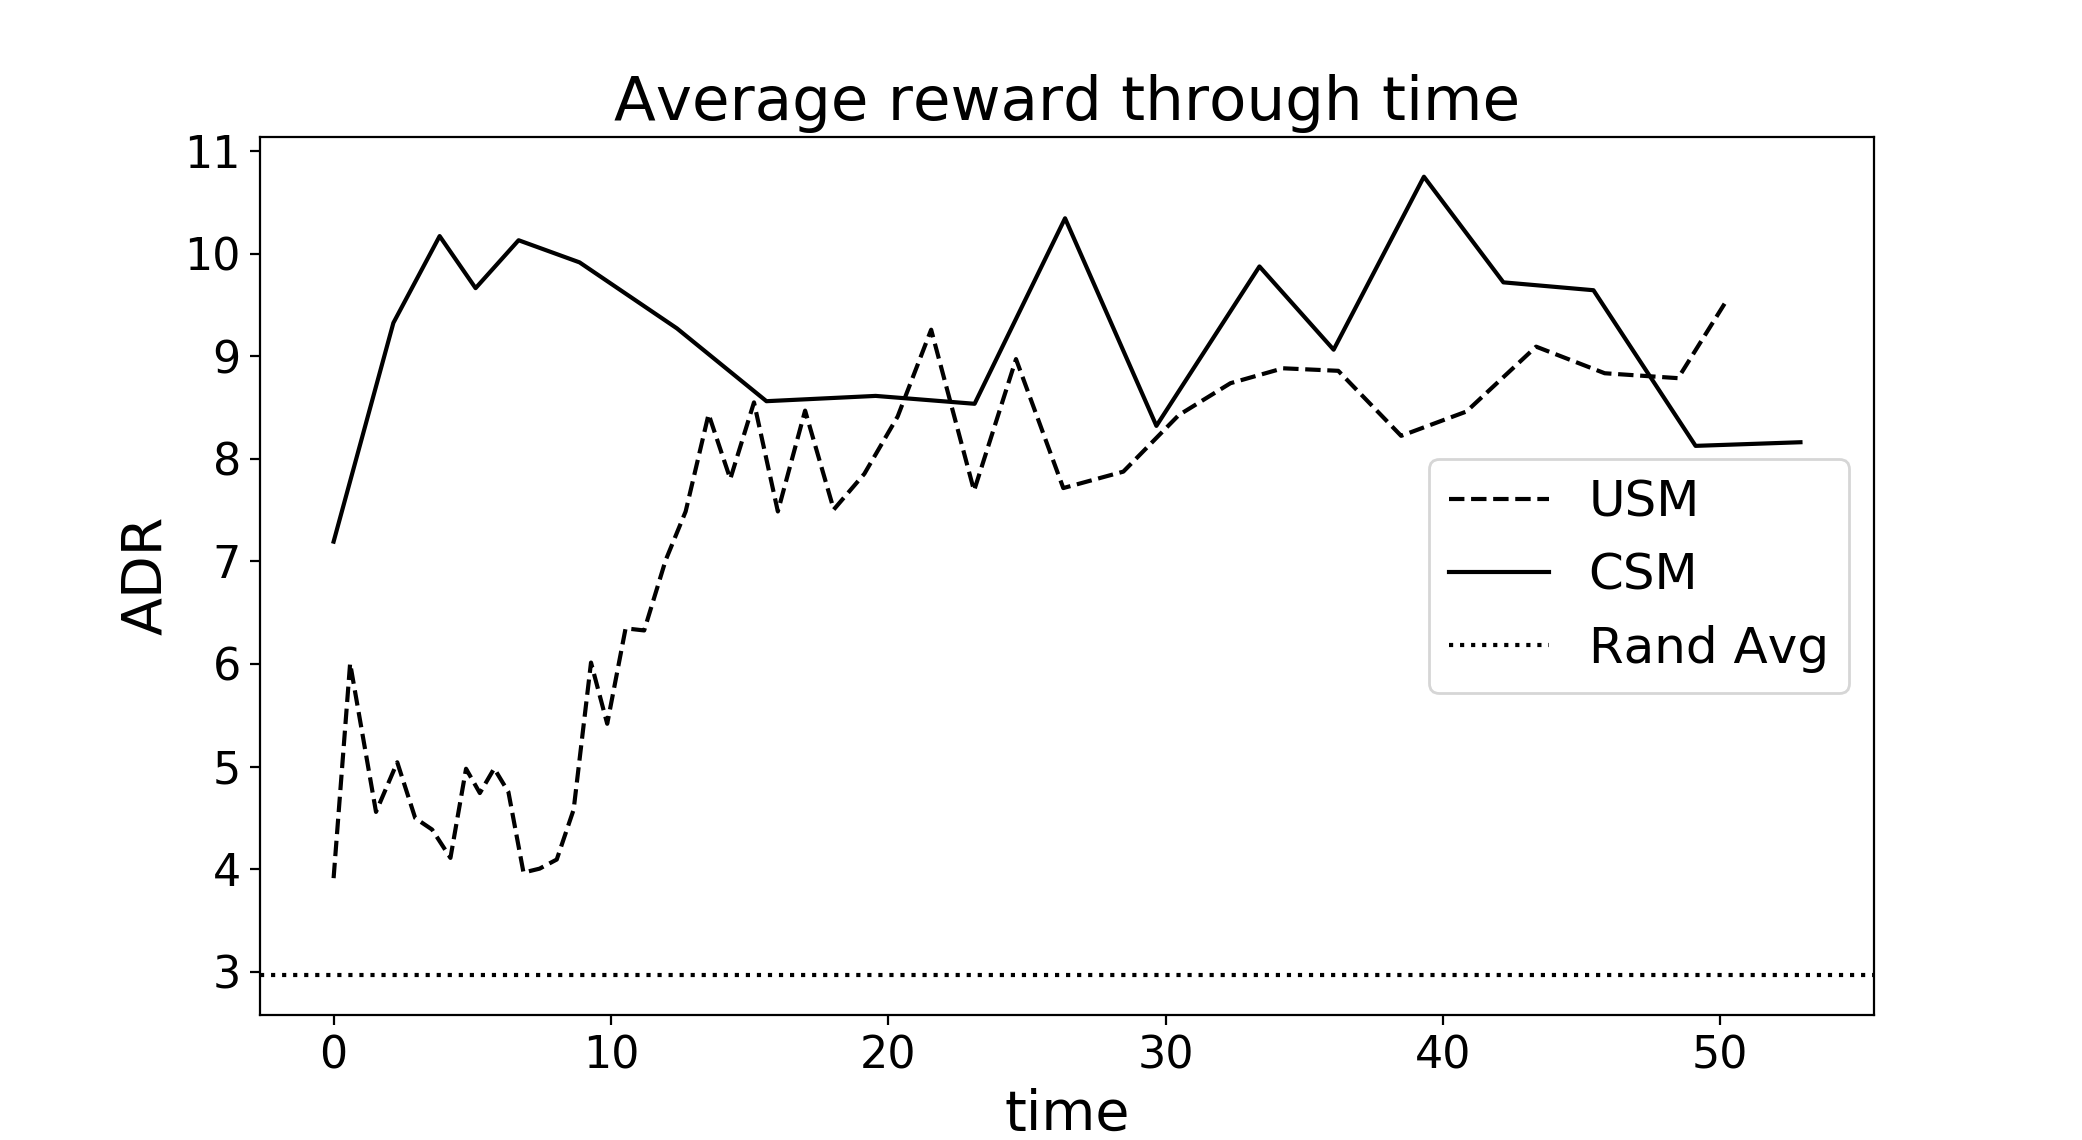
\includegraphics[width=2.8in]{06-13-21-48/hallway_result.png}}\\
 \subfloat[McCallum]{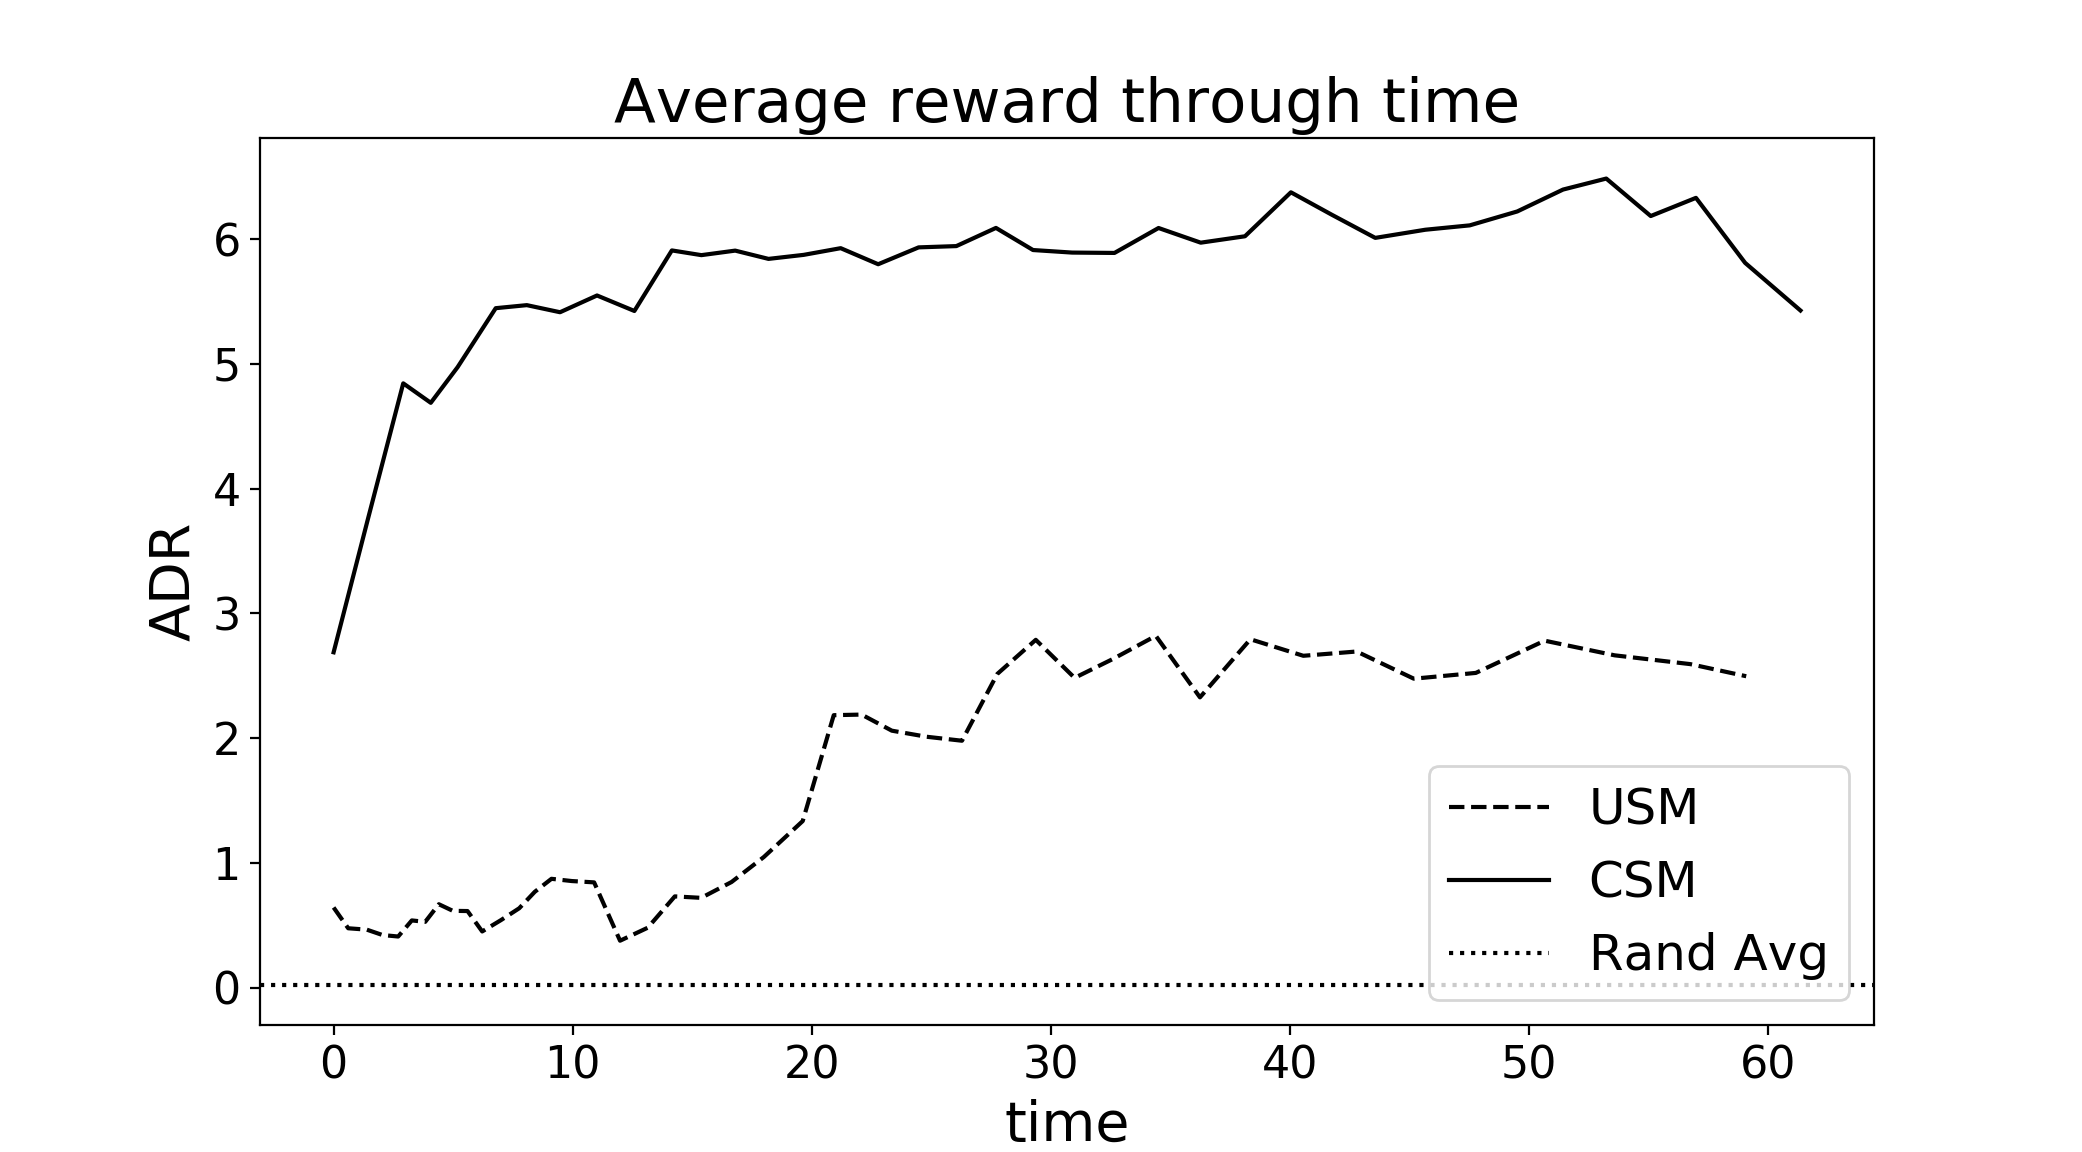
\includegraphics[width=2.8in]{06-13-21-48/mccallum_result.png}}\\
 \subfloat[Prim Maze]{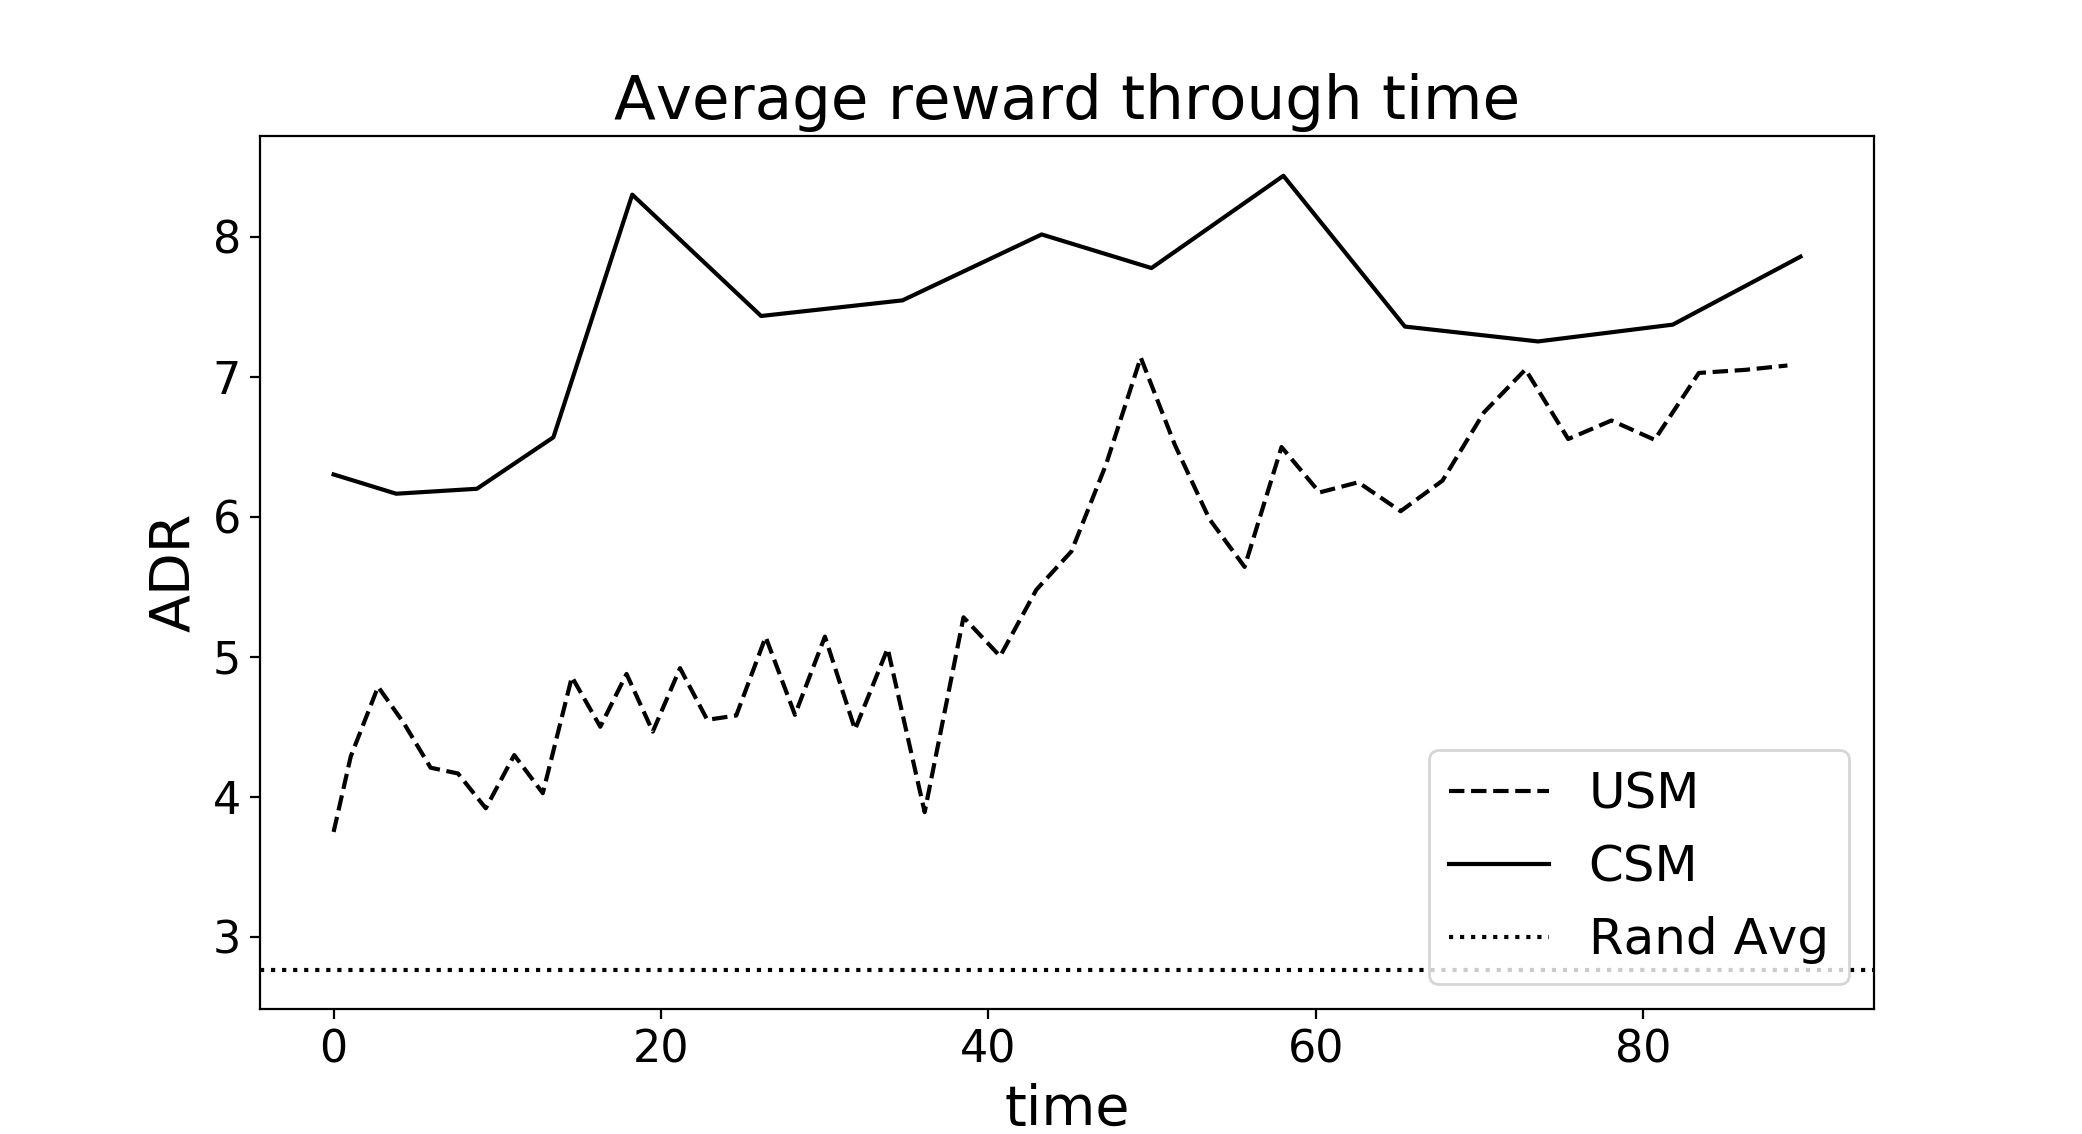
\includegraphics[width=2.8in]{06-13-21-48/prim_maze_result.png}}\\
 \caption{Performance of different agent on different benchmarks; y-axis is $ADR$,
 x-axis is runtime in seconds.}
 \label{fig:agent_adr_time}
\end{figure}

\begin{table}[h]
	\caption{The Comparison of time and $ADR$ between USM and CSM}
	\label{table:results}
	\centering
	\begin{tabular}{lcccc}
		\toprule
                  &\multicolumn{2}{c}{$ADR$}      &\multicolumn{2}{c}{time} \\ 
                  \cmidrule(r){2-3}                 \cmidrule(r){4-5}
    problems      & USM         & CSM               &USM           & CSM      \\
    \midrule
		Tiger-Grid    & 3.81        & 8.70              & 10.75        & 9.45     \\ 
		Hallway       & 8.43        & 10.13             & 13.52        & 6.67     \\ 
		McCallum      & 2.82        & 5.90              & 34.39        & 14.15    \\ 
    Prim Maze     & 7.13        & 8.30              & 49.30        & 18.24    \\ 
    \bottomrule
	\end{tabular}
\end{table}

In Tiger-Grid, CSM algorithm quickly reached a very high $ADR$ in a short
time after the start of the experiment. As the experiment progressed, the $ADR$ of
CSM algorithm converged to 7.5. In contrast, the $ADR$ of USM algorithm fluctuated
drastically in the early stage of the experiment, and became stable at around 4, which
was only half of the CSM algorithm.

In Hallway, the $ADR$ of both algorithms fluctuated violently,  
and converged to a similar value. However, when comparing time taken to reach those,
CSM algorithm reached plateau $ADR$ taken the half runtime of USM algorithm, i.e.,
the agent adopted CSM algorithm have learned twice as fast as agent adopted USM algorithm
in Hallway.

In McCallum, similar to the performance in Tiger-Grid, CSM algorithm quickly reached
a very high $ADR$ in short time after the start of the experiment. As the experiment
progressed, the $ADR$ of CSM algorithm was basically stable at 6. On the other hand,
the $ADR$ of USM algorithm have not significantly increased in the early stage. What's more,
USM algorithm got a far less max $ADR$ than CSM algorithm, which is only about 3. The figure
indicated that in McCallum, CSM algorithm could find a better policy more quickly than USM
algorithm.

In larger scale problems, such as the Prim Maze, CSM algorithm also performed
faster and better than USM. From the experiment results, CSM algorithm achieved an
$ADR$ about 8 in about 20 seconds. USM algorithm, meanwhile, only reached around 5.
Even if in the mid-stage of the experiment, where the $ADR$ of USM has experienced arapid growth,
its time cost was almost three times that of CSM, and had a still lower $ADR$.

In addition, it can be seen from the experiment result that at the beginning of the experiment,
although both algorithms have not gained experience through learning, CSM has obtained a higher
$ADR$ than USM. This can be explained in two ways:
\begin{enumerate}
  \item CSM algorithm uses the Boltzmann sampling method to choose action, the agent does
  not only perform the best action at the stage of exploitation, but  other non-optimal actions,
  which resist overfitting at early stage.
  
  \item CSM rises the $temperature$ of Boltzmann sampling when agent continuously bumps into walls,
  which helps agent get out of that position. That ensures the efficiency of exploration.
  
\end{enumerate}
It is for these two reasons that CSM algorithm is able to understand the environment better and
discover the goal faster than USM algorithm, hence obtaining a higher $ADR$.

Overall, It can be seen that CSM algorithm helps agent to learn faster and better than USM algorithm


\section{Conclusion}

The paper presents an reinforcement learning algorithm to apply heuristic information
into instance-based decision making. We utilized heuristic information in three aspects: constraining the depth
of the suffix tree using L1 distance, densifying instances in tree node according to environment scale 
and utilizing Boltzmann sampling to balance exploration and exploitation. The experiment results
confirmed that CSM algorithm effectively generates good policies, and outperforms USM algorithm in
every benchmark.

In the future work, the computational resources cost by repeatedly suffix matching
is needed to be reduced; time cost of Boltzmann sampling is needed to be reduced.
Furthermore, more effective heuristic standards based on exploration experience have
to be considered. 




% References
\clearpage
\small
\bibliographystyle{named}
\bibliography{dai_2019}


\end{document}
